\documentclass{article}
\usepackage{graphicx} % Required for inserting images
\usepackage{biblatex}
\usepackage{float}
\addbibresource{mybib.bib}

\title{Fall 2024 Photoconductivity Experiment Lab Manual}
\author{Jiakang Xu, Jiakai Li, and Trevor Donovan}
\date{}

\begin{document}

\maketitle


\section{Introduction}
In 1873 English electrical engineer Willoughby Smith discovered that the electrical resistance of selenium varies dramatically with the amount of light falling on it, which is the photoconductivity of selenium, and this is the first discovery of photoconductivity\parencite{Smith73}.The early research about Photoconductivity is limited, focused on the properties of the materials that have the photoconductivity. In the mid-20th century when semiconductor physics was developed, the understanding of photoconductivity was improved significantly. 
The research showed that the photons could excite electrons from the valence band to the conduction band in semiconductors, generating charge carriers and enhancing conductivity. And many materials like silicon, germanium, and cadmium sulfide were studied extensively for their photoconductive properties. The breakthrough of the theory then led to the development of the application. photodetectors, solar cells, and light sensors were invented. The discovery and use of polycrystalline materials and thin films expanded the scope of photoconductive technologies. Nowadays, photoconductivity is used in fields like photovoltaics, imaging technologies, and high-speed communication. 

In this experiment, we used the equipment, Versalab from Quantum Design, to observe the Photoconductivity of Vanadium oxide (VO$_{2}$) by measuring the resistance of VO$_{2}$ with laser shining on and without laser, to find out the influence of the laser to VO$_{2}$.
\section{Photoconductivity}


The phenomenon of photoconductivity (PC) is most clearly observed in semiconductors\parencite{boer23}. A semiconductor is a material that is between the conductor and insulator in ability to conduct. 
In conductors, apart from the completely filled energy bands, there are energy bands that are only partially filled with electrons. These bands can contribute to electrical conductivity and are referred to as conduction bands. In insulators, all energy bands except the filled bands are empty, and these empty bands lack the ability to conduct electricity. In semiconductors, there exists a series of filled bands, with the highest filled band being called the valence band, and a series of empty bands, with the lowest empty band referred to as the conduction band. Between the conduction bands and the valence bands lie bandgaps\parencite{huang1988}.

At a certain temperature or when external energy is applied, some electrons in the valence band can be excited into the conduction band, leaving positively charged electron holes in the valence band. It is also possible that impurities in the semiconductor alter the band filling, resulting in a few electrons in the conduction band and a deficiency of electrons in the valence band, creating holes. Thus, semiconductors conduct electricity through the electrons in the conduction band and the holes in the valence band. The process of the electrons in valence bands are excited to the conduction bands by the external light sources is called photoconductivity. 

%basic PC: generation+recombo rates, steady states, dark vs photocurrent

%intrinsic PC: basic explanation, some eqns.
Intrinsic PC is the process of photons are being absorbed in the valence bands and electrons are excited to the conduction bands, which creates equal numbers of electrons and holes, and is the main cause of photoconductivity in pure semiconductors, which is what we expect for our samples, VO$_{2}$.

%MORE INTRINSIC THEORY.
When the light level is changed in an intrinsic photoconductor, the generation and recombination rates shift and take from picoseconds to tens of nanoseconds to reach a new equilibrium, since intrinsic PC is insensitized. This means we can ignore transient conductivity. Consider an intrinsic photoconductor with dark conductivity $\sigma_0$. The conductivity is proportional to $\mu_nn+\mu_pp$, where n and p are carrier densities of electrons and holes, and $\mu_n$ and $\mu_p$ are their mobilities. Defining $b=\mu_n/\mu_p$, the fractional increase in conductivity due to incident light $\Delta \sigma/\sigma_0$ can be written:

\begin{equation}
    \frac{\Delta \sigma}{\sigma_0} = \frac{\sigma_f-\sigma_0}{\sigma_0} = \frac{b\Delta n+\Delta p}{bn_0+p_0}
\end{equation}

Since $\Delta p = \Delta n$ in intrinsic PC and $p=n$ for pure samples, we can write:

\begin{equation}
    \frac{\Delta \sigma}{\sigma_0} \approx \frac{\Delta n}{n_0}
\end{equation}

In terms of resistances, this can be rewritten:

\begin{equation}
    \frac{R_0}{R_f}-1\approx\frac{\Delta n}{n}
\end{equation}

which allows us to measure the fractional change due to light of charge carriers and conductivity from resistance measurements, without knowing the shape of our samples. Knowing the shape, one can measure the carrier density directly. Note that the light is in general unevenly incident along the surface of the material, so the intrinsic values given here are actually averages.


\section{Experimental Methods}
In this experiment, there are some special methods are used by us and Versalab, which make contribution to the measurements.
\subsection{4-terminal measurements}
The 4-terminal resistance measurements are one of the most common methods for a lock-in amplifier, as shown in figure~\ref{ter}(a)
They have the advantage over simpler methods with two terminals that the 4-terminal resistance measurements remove the effects of contact resistance, as shown in figure~\ref{ter}(b) and \ref{ter} (c)\parencite{Neves24}. In the 2-terminal measurement, the voltmeter measures the voltage of the whole circuit,the voltage of the lead resistance and contact resistance would be part of the measure result. However, in the 4-terminal measurements, the voltmeter is connected in parallel with the sample, so it will only measure the voltage of the sample. The measure result would not be affected by the contact resistance and lead resistance as long as the current is fixed. The Versalab uses 4-terminal measurements to obtain the more accurate resistance measurement values. As shown in the figure~\ref{pin out}, and the table~\ref{interconn}, our sample is only connected to the channel 11-14, We connect the middle two contacts of the sample to channel 13 and 14, and the outer two contacts to 11 and 12, which is the 4-terminal measurement that could remove the lead resistance and lead resistance.
\begin{figure}[H]
    \centering
    \begin{minipage}[t]{0.3\textwidth}
        \centering
        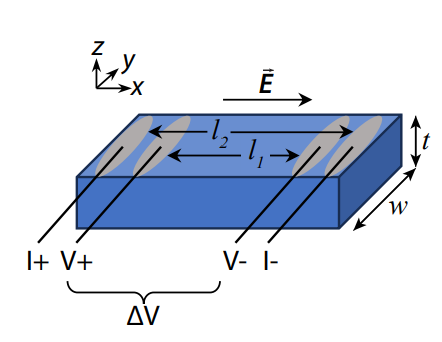
\includegraphics[width=\textwidth]{4tm.png}
       \
    \end{minipage}
    \hfill
    \begin{minipage}[t]{0.3\textwidth}
        \centering
        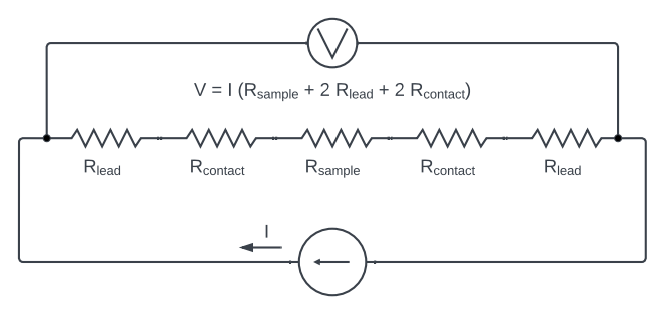
\includegraphics[width=\textwidth]{2tmc.png}
    \end{minipage}
    \hfill
    \begin{minipage}[t]{0.3\textwidth}
        \centering
        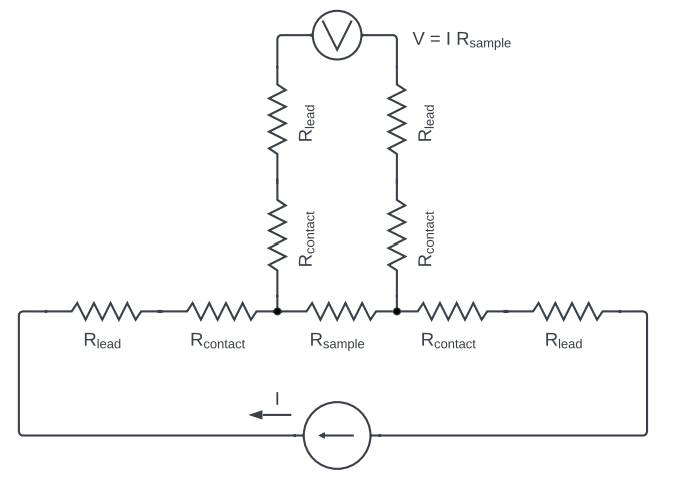
\includegraphics[width=\textwidth]{4tmc.png}
    \end{minipage}
    \caption{(a) The 4-terminal measurement, (b) The 2-terminal measurement circuit, and (c) The 4-terminal measurement circuit  }
    \label{ter}
\end{figure}
\begin{figure}[H]
                \centering
                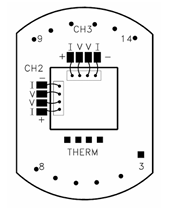
\includegraphics[width=0.25\linewidth]{pin out.png}
                \caption{Pin configuration of resistance bridge sample holder board}
                \label{pin out}
            \end{figure}
            \begin{table}[H]
                \centering
                \begin{tabular}{|c|c|}
                \hline
                   RESISTANCE BRIDGE & RESISTANCE BRIDGE\\
                   BOARD FUNCTION & SAMPLE HOLDER\\
                   \hline
                   Channel 1, I+ & 3    \\  \hline
                   Channel 1, I- & 4    \\  \hline
                   Channel 1, V+ & 5    \\  \hline
                   Channel 1, V- & 6    \\  \hline
                   Channel 2, I+ & 7    \\  \hline
                   Channel 2, I- & 8    \\  \hline
                   Channel 2, V+ & 9    \\  \hline
                   Channel 2, V- & 10   \\  \hline
                   Channel 3, I+ & 11   \\  \hline
                   Channel 3, I- & 12   \\  \hline
                   Channel 3, V+ & 13   \\  \hline
                   Channel 3, V- & 14   \\  \hline
                \end{tabular}
                \caption{Standard interconnection table for sample holder board}
                \label{interconn}
            \end{table}
\subsection{The thin film method}
In the measurement, we use the laser to shine on the sample. To make the sample receive more photons which could excite the electrons, we need to increase the surface area of the sample, which is the shape of thin film. We have two samples in the experiment. The first sample is a strip-shaped solid, and the second sample is a thin film. The measurements also shows that the performance of the thin film is much better than the strip-shaped solid.
\section{Sample}
\subsection{Vanadium(IV) oxide}
Vanadium(IV) oxide is an inorganic compound with the formula VO$_{2}$. It is a semiconductor at room temperature. However, the phase transition occurs around 340K, and VO$_{2}$ transfers from the monoclinic phase, which is semiconducting, to the rutile phase, which is metallic\parencite{Good71}, as the atoms in each pair separate, breaking the localized V-V bonds and releasing the bonding electrons, leading to a sharp increase in electrical conductivity\parencite{Green84}. The temperature of phase transition could be different in heating or cooling; the temperature range in heating is 335-350K, while in cooling it is 340-325K\parencite{Morin59}.The phase transition of VO$_{2}$ can occur in times as short as 100 femtoseconds, which allows it to be extremely fast optical modulators, infrared modulators for missile guidance systems, cameras, data storage, and other applications.  The optical band gap of VO2 in the semiconducting phase is about 0.7 eV\parencite{Shin90}, which is relatively low in semiconductors, meaning its has excellent conductivity.

%\newpage



%%%%%%%%%%%%%%%%%%%%%%%%%%%%%%%%%%%%%%%%%%%%%%%%
%%%%%%%%%%%%%%%%%%%%%%%%%%%%%%%%%%%%%%%%%%%%%%%%
%%%%%%%%%%%%%%%%%%%%%%%%%%%%%%%%%%%%%%%%%%%%%%%%



\section{Equipment}
    
    \subsection{Laser Source}
        In this experiment, we will use two different laser sources of red light. One is a helium-neon laser with $0.95\,mW$ output power (Figure \ref{laser2}). The other produces red light of wavelength 650 nm with 30 mW output power (Figure \ref{laser2}).

        \begin{figure}[H]
        \centering
        \includegraphics[width=0.5\linewidth]{laser 2.jpg}
        \caption{red laser of output power 0.95 mW}
        \label{laser2}
        \end{figure}

         \begin{figure}[H]
        \centering
        \includegraphics[width=0.5\linewidth]{laser 1.jpg}
        \caption{red laser of wavelength 650 nm and output power 30 mW}
        \label{laser1}
        \end{figure}

    \subsection{Quantum Design VersaLab}
        The Quantum Design VersaLab (Figure \ref{Versalab}) is a highly automated flexible instrument designed to measure a variety of the physical properties of a sample while controlling the conditions of the sample chamber: temperature (400 to 50 K), magnetic field (up to 3 T), and atmosphere (atmospheric pressure to high vacuum). VersaLab uses a cryocooler to achieve cryogenic temperatures instead of using liquid cryogens.\\
        Also, VersaLab applies a bias current, which is the excitation, to measure the resistance. Versalab will automatically measure the corresponding voltage and then it will give the value of the corresponding resistance based on $R=\frac{V}{I}$. We can also control the limit of the excitation current, voltage, and its power. Also, we can also use constant current mode (current is fixed at the value we set, and voltage and power control is not available). However, unfortunately, VersaLab does not record or show the value of voltage. The most useful things we need from VersaLab are only the values of excitation current and resistance.

        \begin{figure}[H]
        \centering
        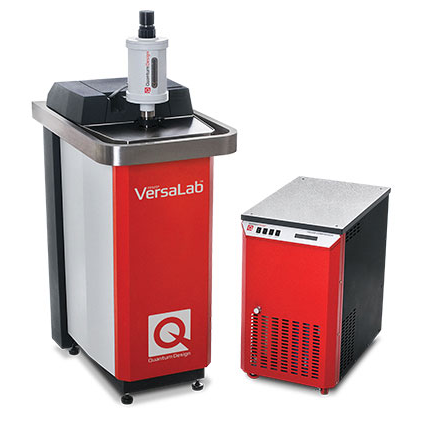
\includegraphics[width=0.75\linewidth]{apparatus pic VersaLab.png}
        \caption{VersaLab}
        \label{Versalab}
        \end{figure}
        
        In order to observe photoconductivity, we need to use a Type A Multi-Function Probe (MFP, Figure \ref{MFP}) which allows connection between itself and a laser source via a light guide fiber (Figure \ref{fiber}). In addition, an adapter is also needed, and its model will vary due to different fibers that you need to use. So, be sure to get a proper adapter, as it will determine if you can have a good connection between the light source and the MFP.\\
        The MFP is also our sample holder where the sample holder board (Figure \ref{sample holder board}) will be installed.\\
        Based on these features of VersaLab, all we need is just to properly mount our sample on a sample holder board, insert the sample holder board into the MFP, and then plug the MFP into VersaLab.\\

        \begin{figure}[H]
        \centering
        \includegraphics[width=0.5\linewidth]{MFP.jpg}
        \caption{Type A Multi-Function Probe (MFP)}
        \label{MFP}
        \end{figure}
        
        \begin{figure}[H]
        \centering
        \includegraphics[width=0.5\linewidth]{Fiber-optic cable.jpg}
        \caption{Fiber-optic cable}
        \label{fiber}
        \end{figure}

        \begin{figure}[H]
        \centering
        \includegraphics[width=0.5\linewidth]{sample holder board.jpg}
        \caption{Sample holder board}
        \label{sample holder board}
        \end{figure}


    \subsection{MultiVu}
    
        MultiVu is a Windows software that allows us to control the operation of the VersaLab hardware and run the measurements, specifically resistivity.\\
        \begin{figure}[H]
            \centering
            \includegraphics[width=1\linewidth]{main menu.png}
            \caption{main menu of MultiVu}
            \label{main menu}
        \end{figure}
        
        In the main menu, you can see a tool bar at the top and a status bar at the bottom. In the status bar, you need to care mainly about the chamber temperature, magnetic field, chamber pressure (Torr), and sequence status. \\
        In order to change these configurations, click "Instruments" in the tool bar shown in Figure \ref{instrument}.Through here, you are able to change magnetic field, temperature, and chamber pressure (in "Chamber option", you can purge or vent the chamber).\\
        Before you try to put in or take out anything the chamber, you must first make sure that temperature is near 300 K, pressure is near atmospheric pressure, namely 750 Torr, and the magnetic field is 0 T. Keep in mind that always first set the temperature at around 300 K before you vent the chamber (Otherwise, the chamber may be full of ice). If these three conditions are met, you can now start to remove probes in the chamber and install the probe you want to use (Read the Sample Installation section for how to install the MFP).\\
        
        \begin{figure}[H]
            \centering
            \includegraphics[width=0.5\linewidth]{instrument.png}
            \caption{instrument configurations}
            \label{instrument}
        \end{figure}

        After you install the MFP physically, you will also need to install the sample in MultiVu. Click "Utilities" in the tool bar and then click "Activate option" (Figure \ref{utilities}). Then, you will see Figure \ref{activate}. Click "Resistivity" in Available Options and then click "Activate". If you want to deactivate something, just click it in Active Options and then click Deactivate.

        \begin{figure}[H]
            \centering
            \includegraphics[width=0.5\linewidth]{utilities.png}
            \caption{Utilities, where you can activate resistivity measurement option}
            \label{utilities}
        \end{figure}

        \begin{figure}[H]
            \centering
            \includegraphics[width=0.75\linewidth]{activate resis.png}
            \caption{activate resistivity measurement for your sample}
            \label{activate}
        \end{figure}

        After success in activating Resistivity, you should be able to see Figure \ref{install sample}. Now, click "Install/Remove" and then follow the instructions that pop up after you click "Install/Remove". When installing the sample, the Versalab will automatically purge the chamber to around 3 Torr (look at the status bar in Figure \ref{Sample installed and sequence editor}). Notice that the box in front of "Installed" has been checked automatically. If not, you can check the bow manually after recalling if you just install or remove the sample.
        
        \begin{figure}[H]
            \centering
            \includegraphics[width=0.5\linewidth]{install sample.png}
            \caption{Install Sample}
            \label{install sample}
        \end{figure}

        Then, click "Browse" in the Resistivity Option" window (Figure \ref{Sample installed and sequence editor}) and select a file with the extension name .dat or you can create a new one so that data can be properly recorded. By clicking "View", you can see the corresponding data graph as shown in Figure \ref{Data graph}. By right clicking the graph, you are able to change the settings of the graph such as xy axis, log scale, and so on.
        
        \begin{figure}[H]
            \centering
            \includegraphics[width=0.75\linewidth]{sample installed and sequence editor.png}
            \caption{Sample installed and sequence editor}
            \label{Sample installed and sequence editor}
        \end{figure}

        \begin{figure}[H]
            \centering
            \includegraphics[width=0.75\linewidth]{data graph.png}
            \caption{Data graph}
            \label{Data graph}
        \end{figure}

        After sample is installed, activate channels by clicking "Bridge setup". You will see Figure \ref{bridge channel}, and just Check the box of Channel 2 and fill in the blanks of current, power, and voltage limit with 10 as we recommend for most time, and then click set. From now on, you can start to measure the resistance or resistivity. The number you should fill depends on the properties of the sample you are measuring. In general, you need restrict the current, power, and voltage so that the current will not burn your sample. Now, try to click "Measure" in "Resistivity Option" window and then you will see Figure \ref{quick measurement}. Check the box of Channel 2 and fill a number you want in the "Readings". Then, click "Measure" at the bottom left and you can see the resistance of your sample at a certain temperature in a while. This is how you do quick measurement at a certain temperature. For instance, if you want to know the resistance of a $VO_{2}$ film only at 380 K, you set the temperature at 380 K and do such quick measurement. This indeed will save you some time. (See Warnings section for why we use channel 2 here.)
        
        \begin{figure}[H]
            \centering
            \includegraphics[width=1\linewidth]{bridge channels.png}
            \caption{bridge channel}
            \label{bridge channel}
        \end{figure}

        
        \begin{figure}[H]
            \centering
            \includegraphics[width=0.75\linewidth]{quick measure.png}
            \caption{quick measurement}
            \label{quick measurement}
        \end{figure}

        Now, you need a sequence to do an automatic measurement. In tool bar, click "File" and create a new sequence. Then, you should be able to see a selected sequence in the "Selected Sequence" window at the left of the main menu. Then, clicking "Edit", you can see the sequence editor in main menu and the "Sequence Commands" window at the right of main menu, as shown in Figure \ref{Sample installed and sequence editor}. By double clicking commands in the "Sequence Commands" window, you can add commands to the sequence editor. You can follow our sequence or design one on your own based on what you need to do. We set an initial temperature with Fast Settles mode before we start the actual measurements. Notice that there is LogData command in the first line of our sequence, you do not have to add this as well because this is usually useless. But if you use this, please remember that the log data file is different from the file you use to record actual data in "Resistivity Option" window. The LogData will only record the systematic status or so-called diagnostic data. Besides, for the actual measurements, we use Uniform, No O'Shoot mode to scan temperature.\\
        At last, save your sequence file and click Run.\\
    
    \subsection{Sample Installation}

            First, by looking at the pin configuration (Figure \ref{pin out}), we find that our measurements will be based on 4-terminal measurements. 4-terminal measurement gives more accurate readings since it separates the current carrying wires from voltage sense wires (see more details in section "4-terminal measurements").\\
            
            Before mounting or wiring the sample, please check the interconnection table (Table \ref{interconn}) and pin configuration. We should use \textbf{Channel 3} on the sample holder board, which refers to Pin 11 to 14. (Notice: we need to activate \textbf{Channel 2} in MultiVu later to start the measurement.)\\
            
            After the sample is mounted, we now plug the sample holder board (with sample mounted) to the corresponding part of the MFP (circled in red in Figure \ref{MFP a red}).

            \begin{figure}[H]
                \centering
                \includegraphics[width=0.5\linewidth]{MFP A red.png}
                \caption{Head of a Type A MFP}
                \label{MFP a red}
            \end{figure}

            Then, use puck insertion tool (Figure \ref{puck tool}) to take out the puck inside the VersaLab chamber. The lever of the puck-insertion tool is engaged when it is lying flat across the handle, as is shown in Figure \ref{tool engaged}. When the lever is engaged, the tool grips the puck. Besides, you can also use this tool to install a puck. However, we are not going to use a sample puck in this experiment. You need to use this tool just in case others use a sample puck and leave the puck inside the chamber. A sample puck is a cylinder object as shown in Figure \ref{puck}. It may be either a short or long cylinder.

            \begin{figure}[H]
                \centering
                \includegraphics[width=0.75\linewidth]{Puck Insertion Tool .jpg}
                \caption{Puck insertion tool}
                \label{puck tool}
            \end{figure}

            \begin{figure}[H]
                \centering
                \includegraphics[width=0.75\linewidth]{puck.png}
                \caption{A sample puck}
                \label{puck}
            \end{figure}

            \begin{figure}[H]
                \centering
                \includegraphics[width=0.25\linewidth]{tool engaged.png}
                \caption{operation of puck insertion tool}
                \label{tool engaged}
            \end{figure}
            
            Now, we install the MFP into the Versalab chamber as shown in Figure \ref{MFP install}. Be sure that you move the MFP smoothly and the O-ring (Figure \ref{O-ring}) sits steadily in the groove on the ferrule of the chamber. Once the MFP reaches the end of the chamber, rotate the MFP slowly until you feel a click. Then, press the MFP a little bit so that the MFP sits steadily in the chamber and can not be rotated any more. Then, attach and tighten the clamp to the ferrule so that the chamber is certainly sealed. If you succeed installing the MFP, you should be able to see Figure \ref{MFP installed}. (Plus: Here we already attached the fiber.)
            
            \begin{figure}[H]
                \centering
                \includegraphics[width=0.75\linewidth, angle=270]{MFP install.jpg}
                \caption{MFP installation}
                \label{MFP install}
            \end{figure}

            \begin{figure}[H]
                \centering
                \includegraphics[width=0.75\linewidth, angle=270]{MFP installed.jpg}
                \caption{MFP installed}
                \label{MFP installed}
            \end{figure}

            \begin{figure}[H]
            \centering
            \includegraphics[width=0.5\linewidth]{O ring.jpg}
            \caption{O-ring}
            \label{O-ring}
            \end{figure}

            Now, we need to install the BRT module (Figure \ref{BRT}) which is designated for resistivity measurements.\\
            Look at the panel (Figure \ref{panel}) and find the ports, BRIDGE JL-1 and TEMP JL-3, and then connect the wires of BRT module (Figure \ref{BRT}) to the two ports. Then, connect the BRT module to VersaLab as shown in Figure \ref{BRT install}. Keep in mind that you always align the red dots on BRT module and the panel and that you will not feel resistance if all red dots are aligned when you install the BRT.\\

            \begin{figure}[H]
                \centering
                \includegraphics[width=0.5\linewidth]{BRT module.jpg}
                \caption{BRT module}
                \label{BRT}
            \end{figure}

            \begin{figure}[H]
                \centering
                \includegraphics[width=0.75\linewidth]{panel.jpg}
                \caption{Panel on VersaLab}
                \label{panel}
            \end{figure}

            \begin{figure}[H]
                \centering
                \includegraphics[width=0.75\linewidth]{BRT install.jpg}
                \caption{BRT installation. The output channels (which match the sample puck channel labels) correspond to different output channels (which match the MultiVu channel labels). For example, the $\mathrm{VO_2}$ puck uses its channel 3 connections, so MultiVu sequences must measure "Channel 2".}
                \label{BRT install}
            \end{figure}

            Now, it is time to connect the laser source to the MFP by a fiber-optic cable (Figure \ref{fiber}). This is an easy work.\\

            Now, start your measurement on MultiVu.
            
    \subsection{Sample inspection}

    In order to see if your sample is wired correctly, you can use the puck-wiring test station (Figure \ref{station1} and Figure \ref{station2}). You just need to put your sample holder board on the test station and use a digital multimeter to check the resistance between any two of the channels. Also, you can use a magnifier to see how the sample is wired.

        \begin{figure}[H]
        \centering
        \includegraphics[width=0.5\linewidth]{Puck-wiring Test Station 1.jpg}
        \caption{puck-wiring test station}
        \label{station1}
        \end{figure}

        \begin{figure}[H]
        \centering
        \includegraphics[width=0.5\linewidth]{Puck-wiring Test Station 2.jpg}
        \caption{puck-wiring test station}
        \label{station2}
        \end{figure}

    \subsection{Warnings}
        \subsubsection{Always leave MultiVu open}
            If MultiVu is left closed for more than 5 consecutive minutes, the system automatically shuts down both the magnet and temperature control, so the chamber temperature will start to drift down and usually settles at ~200K if left in that state long enough.
        
        \subsubsection{Procedures to open the chamber}
            1. Set the chamber temperature at 300 K.\\
            2. After the temperature is steady around 300 K, vent the chamber.\\
            3. Set the magnetic field at 0 T.\\
            4. Deactivate the measurement option that you are using now.\\
            5. Take whatever inside the chamber out.\\
        \textbf{Always follow these steps. Otherwise, the chamber might be frozen.}\\

        \subsubsection{Do not tighten the clamp too much when you insert the MFP into the chamber}

        \subsubsection{BRT module redirects the channels of the sample holder board}
            If you wire the sample on channel 2 (respectively, 3) of the sample holder board, you should use channel 1 (respectively, 2) on MultiVu. So, be careful which channel you are using and do not use the wrong channel.
    



%%%%%%%%%%%%%%%%%%%%%%%%%%%%%%%%%%%%%%%%%%%%%%%%
%%%%%%%%%%%%%%%%%%%%%%%%%%%%%%%%%%%%%%%%%%%%%%%%
%%%%%%%%%%%%%%%%%%%%%%%%%%%%%%%%%%%%%%%%%%%%%%%%






\section{Necessary Improvements}

This section is not entirely intended for the manual as will be shown to students, but rather to advocate for certain additions to the experimental setup. We were unable to measure photoconductivity with the VersaLab setup as we had it. When the laser illuminated the sample, the thermal effect played a significant (probably dominant) role in increasing the conductivity, which could not be decoupled from direct carrier generation.

We may be able to measure photoconductivity if we can interface an optical chopper and a lock-in amplifier with the VersaLab. A 2015 article described a success in isolating photoconductivity in vanadium dioxide nanowires using these two devices \parencite{wang2015}. Since the thermal effect is much slower-acting than the extremely fast direct excitation, light chopped at high frequency (a few thousand Hertz as an example from the paper), diminishes the thermal effect greatly, leaving the photoexcitation which occurs at the chopping frequency.

Since the chopper causes our desired effect to occur at a specific frequency, we want to isolate and amplify effects at that frequency from others. A lock-in amplifier works by repeatedly integrating an input signal multiplied with a sinusoidal reference signal, which by the orthogonality of sinusoids cancels out most frequency components except the one matching the reference. The lock-in amplifier would also greatly reduce noise. The reference and input phases must also match \parencite{aboutLIAs}. For complicated signals, this means one can extract the orthogonal sine and cosine components of a signal at a given frequency and determine the magnitude of that frequency's (amplified) Fourier coefficient. Finding a way to install a chopper and lock-in amplifier to the VersaLab optical input and measurement system may allow us to use its sequence functionality to make autonomous measurements of direct-excitation photoconductivity at wide temperature and magnetic field ranges.

In the following sections, we lay out an observation and analysis plan assuming an optical chopper and lock-in amplifier are available and can be installed in the setup.

%%
%Throw out + replace most of the analysis section, re-scrutinize the measurement section.
%%

\section{Measurements}

You will have about 8 3-hour class sessions over a period lasting a month to take measurements, do analysis, and hand in your paper. This experiment demands a number of long, autonomous measurements, so you may only need to be present at the beginning of most class periods, but it is your choice. Use that extra time to write the necessary code to do analysis on data as it is acquired.

The primary goal of this experiment is to measure the photoconductivity of a few sample materials. A supplementary goal of this experiment is to measure the dependence of conductivity or resistivity on quantities such as temperature, magnetic field, and previous sample state (hysteresis).

We will use the VersaLab to provide the precise temperature and field control, and chopped laser light coupled to into the multifunction probe (see Fig. \ref{MFP}) to excite photoconductivity modulated in time. With a chopping frequency of a few kHz, this allows us to address the problem of heating the sample, since the thermal effect is a low-frequency process.

%\begin{figure}
%    \centering
%    \includegraphics[scale=.3]{multif_probe.png}
%    \caption{The VersaLab's multifunction probe. It allows fiber-%coupled light (from the top portion shown left, with a fiber running %through the central bar) to illuminate the sample mounted on the %green device shown right.}
%    \label{fig:multifunction_probe}
%\end{figure}


Before beginning the measurements sequence, make sure the resistivity option is activated and the pressure is low (around a few Torr). For laser measurements, make sure the laser is actually on before measurements begin and will not shut off. The fault locator laser has a battery life of about 10 hours(long enough for a long measurement, but not two or three), so it may be necessary to replace it before each long measurement. 

%\begin{figure}
 %   \centering
 %   \includegraphics[scale=.23]{multivu_demo_image.png}
 %   \caption{The MultiVu user interface, which allows the creation, %operation, and display of measurement sequences, graphs, and data %files. The Option Manager is available from "Utilities" above. %Click "Resistivity" then "Activate" to activate the resistivity %measurement option. This will create an option for the %Resistivity command when writing a sequence which must be used to %measure resistances.}
%    \label{fig:resistivity_option_multivu}
%\end{figure}

When writing sequences, make sure to adhere to the following guidelines. Since the setup will be sitting for a while at the end of the sequence before anyone touches it again, it is ideal to set the temperature to 300 Kelvin at the end of the sequence. To measure the expected temperature hysteresis and compare to materials without it, the sequence must sweep up and down in temperature. Keep track of which direction (hot to cold or cold to hot) happens first, as you may want to separate these sections in the analysis. Note that though you are measuring resistances, MultiVu calls the measurement resistivity because it is made with an assumed sample shape in mind. Our samples are in general less regularly shaped, so make sure to select Ohms as the unit of measurement.

If the voltage, power, or current limits are met during the course of a measurement, split the sequence into two (or four, if it goes in both directions in temperature) temperature sweeps with appropriately adjusted voltage, power, and current limits. This (in addition to broken sample wiring) is a likely solution to any flat sections of graphs that occur at the temperature extremes.

A suggested measurement schedule is given below, designed to require 6 class periods of measurement. More time may be necessary in later class periods or outside of class, or one of the three sample materials can be skipped if time requires.

\begin{itemize}
    \item \textbf{Class 1:} Familiarize yourselves with using the VersaLab and MultiVu setup with the chopper and amplifier components safely and as intended, using the TA, instructor, and manuals as reference resources whenever something about the setup is unsure. First, test out a single resistance measurement of a sample of known resistance to verify which channels to use (see Fig. \ref{BRT install} for an explanation of channels). Then, write a practice sequence to measure this repeatedly and save the data to a file, sweeping over small temperature and magnetic field ranges (keeping in mind that the chamber temperature will actually change much slower than the rate given in the sequence), and check that the data file is produced correctly. Note that the VersaLab and MultiVu have no built-in uncertainty estimation. Use a sequence or repeated single-measurements to build statistics at a few temperatures to estimate the uncertainty on a temperature measurement. Finally, if everything has gone correctly, replace the known sample with the vanadium dioxide sample, then write and start a sequence that sweeps temperature from 200-400 Kelvin and back, also sweeping through a small number of magnetic field values at each temperature. Make sure the temperature points are more than finely spaced enough to measure the expected drop or rise in resistivity, but try to keep the expected duration less than 10 hours.
    \item \textbf{Class 2:} After securing the data from the previous class's acquisition, repeat class 1's measurement but with a bright laser fiber-coupled to the probe. In order to create the proper bias of charge carriers, make sure the light is not shining uniformly on the sample. If the light is not chopped and measured in the frequency domain with a lock-in amplifier, it is uncertain how much of the effect is from direct excitation as opposed to thermal excitation.
    \item \textbf{Class 3-6:} Repeat the above, but for the two other samples (gallium arsenide and indium arsenide)
\end{itemize}

%\begin{figure}
%    \centering
%    \includegraphics[scale=.07]{channels.jpg}
%    \caption{}
%    \label{fig:channels}
%\end{figure}

Assuming we are still using MultiVu's data acquisition for a given measurement instead of third-party measurements associated with the amplifier: Once a given measurement is done, the data will be saved to the file specified in the sequence. Copy the .dat files (e.g. by using a portable hard drive) to your computers. Each data file contains a header by default, which matters because it is preferable to convert the .dat files to .csv files by simply changing the file handle of the data files. Before converting the file type, you must delete this header so the top row of the .csv file is made of strings and each line below is made of numbers. After you have these .csv files(which can be checked for correctness in a program such as Jupyter Notebook), you are ready to analyze the data.

\section{Analysis}

Assuming analysis is done in Python: It is recommended that (for each student) the analysis be done in a program such as Jupyter Notebook or Visual Studio Code with many sequential blocks of code in one file. Modules such as pandas (by converting .csv files to the malleable dataframe object type and making use of their many sorting and selecting functions), Numpy (for handling any arrays of numbers in typically more familiar ways than pandas), SciPy (for fitting curves to data and doing all statistics), and Matplotlib (for visualizing data) will prove useful for analysis.

Whenever you acquire the data for a relation of any sort, plot it first. Given the multiple variables at play in these measurements, think carefully about how and what to plot to most transparently communicate the important details of the data. Fit curves to the data to determine graph statistics.

How isolated is the direct excitation from the thermal excitation? How accurate are the temperatures given by MultiVu to the temperature of the conductive parts of the samples?

It is resistance or conductance that is directly measured, but we are interested in resistivity or conductivity. Can you model the shape of the sample to determine conductivities from the measured resistances? Can you estimate the carrier number and carrier density due to temperature, magnetic field, and photoconductivity?

\section{Results during experiment development}

This section is not intended for the manual as will be shown to students. It is just a showcase of some of our results from the semester.

Our first $\mathrm{VO_2}$ sample was irregularly shaped, unstable, and may have broken and changed its structure at least once due to temperature stress, as suggested by Fig. \ref{fig:first_vo2_graph}. The contact resistance from the wires attached to the sample may also have been significant.

\begin{figure}
    \centering
    \includegraphics[scale=.7]{first_vo2.png}
    \caption{Resistivity vs. Temperature for our first vanadium dioxide sample. The orange and blue data were taken in succession, and the green data were taken (with increasing temperature) at a different time. A phase transition with hysteresis is confirmed, but the data are noisy and change significantly between runs.}
    \label{fig:first_vo2_graph}
\end{figure}

The vanadium dioxide sample was replaced as a result of these issues, and the resulting graph shown in Fig. \ref{fig:second_vo2_graph}. We also acquired a laser and the equipment to fiber-couple, so we graph laser-lit and dark data.


\begin{figure}
    \centering
    \includegraphics[scale=.7]{second_vo2.png}
    \caption{Resistivity vs. Temperature for our second vanadium dioxide sample. These graphs are much less noisy than before, indicating a sample and connections of higher quality. The dark graphs consistently have higher resistances than the corresponding laser-lit graphs in the insulating regime, which is caused by a mix of direct excitation and thermal excitation in uncertain proportions.}
    \label{fig:second_vo2_graph}
\end{figure}

To compare the dark graphs to the light graphs in more detail, we divide and subtract them as shown in Fig. \ref{fig:vo2_dark_light}.

\begin{figure}
    \centering
    \includegraphics[scale=.4]{vo2_dark_light_comparison.png}
    \caption{Left: Resistance differences show that dark resistance is higher below transition temperature and that dark and lit resistances tend to become more similar as temperature increases, except when the phase transition begins. Right: The resistance ratio graphs show that dark resistance is a little lower above transition temperature. The downward spikes show that the sample transitions at lower chamber temperature when lit, meaning the laser is meaningfully changing the temperature. The laser's influence on the crystal transition is evidence of the unwanted thermal effect.}
    \label{fig:vo2_dark_light}
\end{figure}

Note that these are preliminary results and have no uncertainty on them because finding uncertainties was not a priority in developing the experiment. Also, at this point, it had become known that the measurement could not be completed without a chopper and a lock-in amplifier. More data (which is not meaningfully different from the results shown in this section) was taken with different combinations of lasers and current/power/voltage limits, but we now know it will not display photoconductivity separately from light-induced thermal conductivity.


\section*{Section Authors}
Jiakang Xu wrote the Introduction, Experimental Methods, and Sample sections, and edited the Photoconductivity section. Jiakai Li wrote the extensive Equipment section. Trevor Donovan wrote the Necessary Improvements, Measurements, Analysis, and Results during experiment development sections, and wrote the original, unedited Photoconductivity section.

\printbibliography

\end{document}
